%%%%%%%%%%%%%%%%%%%%%%%%%%%%%%%%%%%%%%%%%%%%%%%%%%%%%%%%%%%%%%%%%%%%%%%%%%%%%%%%%%%%
% Do not alter this block (unless you're familiar with LaTeX)
\documentclass{../labbook}

%%%%%%%%%%%%%%%%%%%%%%%%%%%%%%%%%%%%%%%%%%%%%
%Fill in the appropriate information below
\lhead{Group lab 1}
\rhead{Speech Synthesis I} 
\chead{\textbf{ Due: \textbf{WED 13.12.2023 23:59} CET}}
%%%%%%%%%%%%%%%%%%%%%%%%%%%%%%%%%%%%%%%%%%%%%

\begin{document}
\begin{mdframed}[backgroundcolor=blue!20]
\LaTeX ~submissions are mandatory. Submitting your assignment in another format will be graded no higher than R.
\end{mdframed}

%%%%%%%%%%%%%%%%%%%%%%%%%%%%%%
\section{Group members}
Weihao Jiang, Chenyu Li, Yanhua Liao, Cantao Su, Yinqiu Wang
%%%%%%%%%%%%%%%%%%%%%%%%%%%%%%

\section{Group lab TTS 1.}
In this group lab you will do an exploration of different pitch trackers.

\subsection{Submission}
For this submission you will need to commit the LaTeX file as usual, as well as plots of $f_0$. Therefore, the completed commit for this assignment includes:
\begin{enumerate}
    \item LaTeX file that includes the plots and your reflections.
    \item Your code (you commit your code file alongside your LaTeX file).
    \item Plots (you commit your plots alongside your LaTeX file).
    \item Audio recordings you used for the task (you commit them alongside your LaTeX file).
\end{enumerate}

\subsubsection*{Preparation:}

You will need to \underline{extracting F0 using different pitch trackers}. 

There are quite a few free (as “libre” in “gratis vs libre”) implementations of pitch tracking algorithms. Let’s try out some:
\begin{itemize}
    \item \textbf{Praat} (you are already very familiar with the tool)
    \item \textbf{YIN} (Name is from ‘‘yin’’ and ‘‘yang’’ of oriental philosophy. De Cheveigné, \& Kawahara, 2002).     
    
    How to: \href{https://librosa.org/doc/main/generated/librosa.yin.html}{https://librosa.org/doc/main/generated/librosa.yin.html}
    
    \item \textbf{RAPT} (Robust Algorithm for Pitch Tracking. Talkin \& Kleijn, 1995)
    
    How to: \href{https://pysptk.readthedocs.io/en/latest/generated/pysptk.sptk.rapt.html}{https://pysptk.readthedocs.io/en/latest/generated/pysptk.sptk.rapt.html}
    
    \item \textbf{SWIPE} (Sawtooth Waveform Inspired Pitch Estimator. Camacho \& Harris, 2008)
    
    How to: \href{https://pysptk.readthedocs.io/en/latest/generated/pysptk.sptk.swipe.html}{https://pysptk.readthedocs.io/en/latest/generated/pysptk.sptk.swipe.html}

    \item \textbf{REAPER} (Robust Epoch And Pitch EstimatoR. Talkin, 2015). 
   
    How to: go to \href{https://github.com/google/REAPER}{https://github.com/google/REAPER} and follow the instructions. You may need a C compiler and other basic stuff (in deb-based systems do apt install build-essential)

    \item \textbf{YAAPT} (``yet another algorithm for pitch tracking''. Zahorian \& Hu (2008).) 
    
    How to: \href{https://github.com/bjbschmitt/AMFM_decompy/blob/master/amfm_decompy/pYAAPT.py}{the code for pYAAPT.py can be found as part of "AMFM decompy" package}
(here is a link to \href{https://github.com/bjbschmitt/AMFM_decompy/}{AMFM decompy python package})
\end{itemize}

\underline{Data to use}.

You will need several files for your group lab: together with your group members decide on several audio files, maximum five. These recordings should not be longer than just one sentence, so it would be easier for you to compare later.
These files should have different acoustic environments and/or speaking styles (consider including audio files that differ in phonation types, like breathy or creaky speech). 
You can either reuse the recordings you made/used for the previous classes or record new ones.

\begin{problem}{1}{10}{Plotting F0 and reflecting on the results}

\subsubsection*{Task:}

\begin{enumerate}
    \item Select at least three pitch tracking algorithms you will work with.
    \item Get text files with F0 values generated by different algorithms (with the same pitch range settings).
    \item Plot the F0 values for every file you selected. 
    \item Compare the graphs for each algorithm.
    \item Reflect on what you see on these plots: do you see any errors that pitch tracker(s) made? do plots differ in any way for any of the files you included in your test set of recordings? Speculate on the reasons if you see errors and/or differences.
    Based on your exploratory visual analysis, explain which algorithm would you chose to use and why.
   
\end{enumerate}

\end{problem}

%%%%%%%%%%%%%%%%%%%%%%%%%%%%%%%%%%%%%%%%%%%%%
\begin{solution}

\textbf{Normal speech:}
\begin{figure}[h]
    \centering
    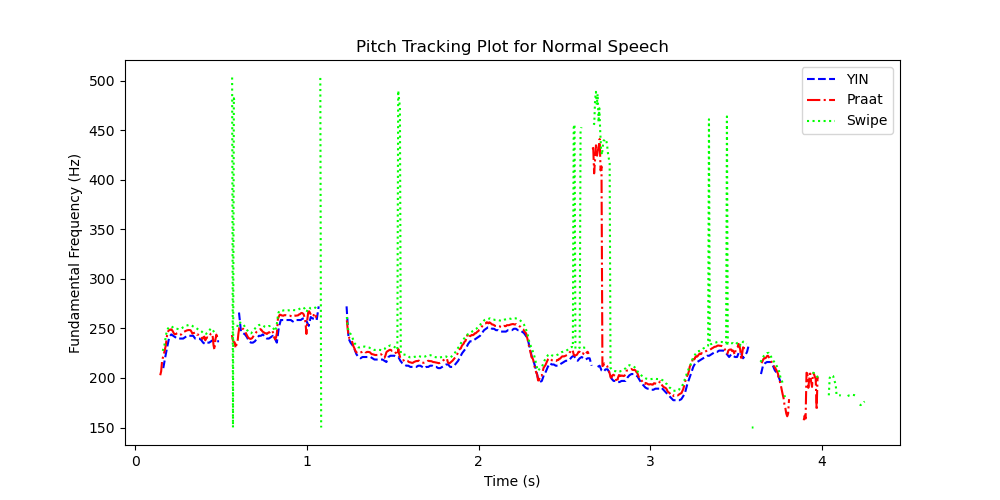
\includegraphics[width=0.8\linewidth]{recording1_normal_fm_pitch_plot.png}
    \caption{Normal Speech}
    \label{Normal Speech}
\end{figure}

\textbf{Observations:}
\begin{itemize}
    \item \textbf{Praat's plot:} The overall output of the algorithm is more stable and smooth, showing the F0 direction of the audio signal. However, by looking at the picture, we see that high frequency values suddenly appear in the middle of the 2nd and 3rd seconds. But by checking the same time points in the recording, there is no abnormal sound or signal in the recording   

    \item \textbf{SWIPE's Plot:} Compared to the output of Praat and YIN, SWIPE shows a lot of high frequency values. We speculate that the algorithm design of SWIPE may be very sensitive to small fluctuations in the audio signal. Some algorithms may be designed to over-respond to or amplify high-frequency noise or fluctuations in the signal, resulting in many high-frequency values seen in the output.

    \item \textbf{YIN's Plot:} The output of this algorithm is the most silky and stable of the three algorithms. The trend of the overall signal's F0 over time can be seen in the picture. There are hardly any outlying high frequency values. We speculate that perhaps the YIN  algorithm is more robust, and perhaps this algorithm is more complex in design and therefore more fault tolerant compared to the other two algorithms.

\end{itemize}

\textbf{Summary:} In the analysis of pitch tracking algorithms, Praat and YIN show closer results, while the differences are more pronounced for SWIPE. Therefore, it is recommended to use the algorithm YIN in recordings with minimal noise and a stable speaker state, as it is effective in capturing the overall trend and occasional high frequencies, and shows an overall stable performance. However, SWIPE is least recommended due to its more unstable performance.\\

\textbf{Quiet speech:}
\begin{figure}[h]
    \centering
    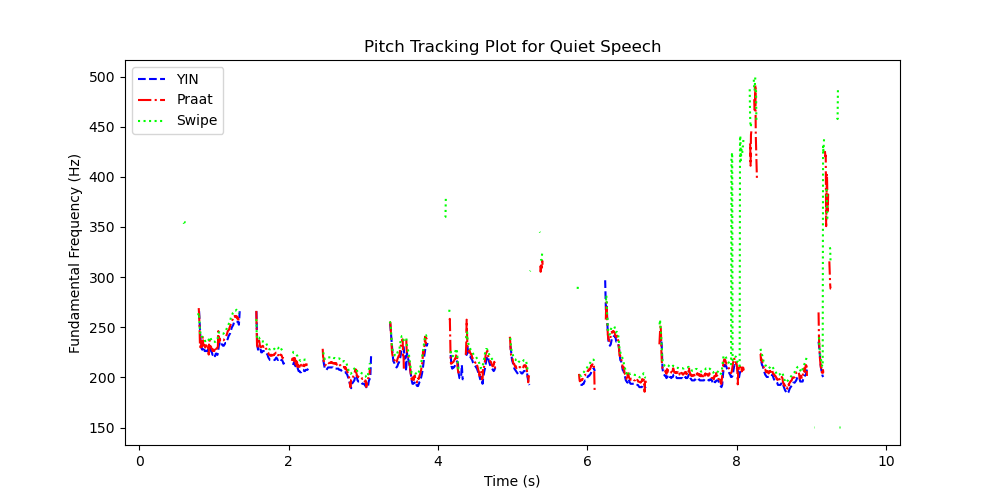
\includegraphics[width=0.8\linewidth]{recording2_quiet_fm_pitch_plot.png}
    \caption{Quiet Speech}
    \label{Quiet Speech}
\end{figure}

\textbf{Observations:}
\begin{itemize}
    \item \textbf{Praat's plot:} The pitch contour of Praat appears relatively stable compared with others, with the exception of a sudden increase from 200 to 400 Hz between 8 to 10 seconds. Upon re-listening to the audio, it was observed that the speaker significantly stressed the word "wrapped" during this time frame. Hence, the sudden upward shift in pitch during this interval is considered a normal phenomenon, indicating that the algorithm accurately captures variations in pitch. Overall, Praat exhibits fewer outliers, and its pitch contour is relatively similar to that of SWIPE, with occasional outliers that are also relatively close to the pitch contours of the other two algorithms.


    \item \textbf{SWIPE's Plot:} SWIPE exhibits a lot of variations and some outliers, indicating its relatively higher sensitivity compared to the other two algorithms. Additionally, it shows significant differences from the other two algorithms in certain areas. For instance, in the 0-5 seconds interval, the SWIPE algorithm extracted some outliers in the range of 300-500 Hz, whereas the other two algorithms did not detect pitch variations in those regions. Therefore, it can be inferred that errors are more likely to occur in SWIPE.


    \item \textbf{YIN's Plot:}The YIN algorithm is the most consistent and stable among the three algorithms, but this also indicates that the YIN algorithm is not as sensitive in capturing pitch variations. For example, at 5-6 seconds and 8-10 seconds, Praat and SWIPE detected changes in pitch, whereas the YIN algorithm did not capture these variations.

\end{itemize}

\textbf{Summary:} In general, it can be observed that SWIPE has the highest number of outliers, suggesting that SWIPE may be more sensitive among the three algorithms and could potentially confuse noise and breathiness. The pitch contour extracted by the YIN algorithm is the smoothest, indicating that the algorithm may not capture certain subtle variations in pitch. Therefore, overall, in a quiet environment, I would prioritize choosing the Praat algorithm as it is relatively more stable compared to SWIPE and more sensitive compared to YIN, so the pitch contour extracted using Praat should be the most accurate in the end.\\

\textbf{Breathy speech:}
\begin{figure}[h]
    \centering
    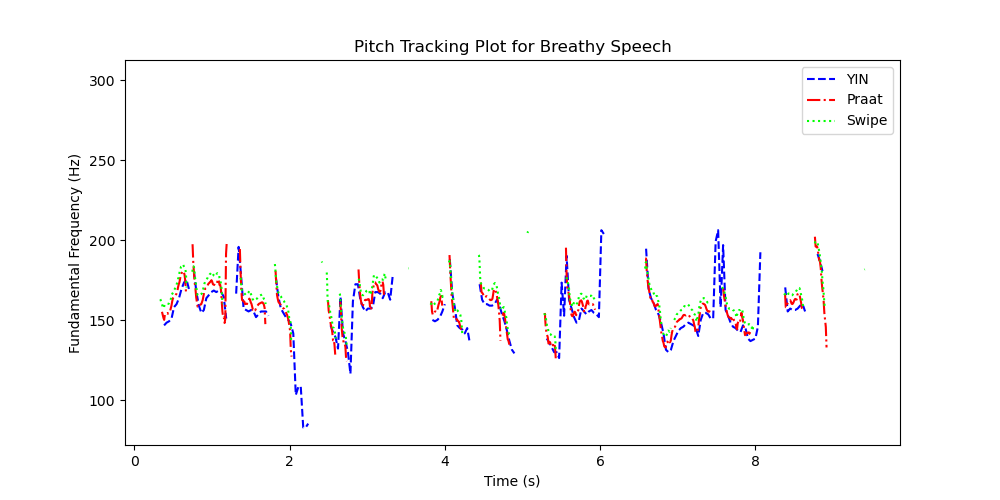
\includegraphics[width=0.8\linewidth]{recording3_breathy_m_pitch_plot.png}
    \caption{Breathy Speech}
    \label{Breathy speech}
\end{figure}

\textbf{Observations:}
\begin{itemize}
    \item \textbf{Praat's plot:} The pitch contour detected by Praat still appears relatively stable and consistent, similar to its performance with quiet speech. It manages to maintain a smooth contour with fewer fluctuations than the other algorithms, suggesting robustness against the breathy quality of the speech, which can often introduce noise into the pitch tracking process.



    \item \textbf{SWIPE's Plot:} SWIPE generally performs well in recognizing F0 in breathy speech, with overall numerical consistency comparable to values identified using Praat. However, the main issue with SWIPE is the occurrence of some disjointed and sudden outliers in its plot.



    \item \textbf{YIN's Plot:}The pitch tracking in YIN's plot exhibits greater variance compared to the quiet speech plot, suggesting a heightened sensitivity to pitch deviations, possibly influenced by the breathiness of speech. Despite the elevated variance, YIN demonstrates good overall coherence, as there are no abrupt, disjointed data points present in its graph.

\end{itemize}

\textbf{Summary:} In the recognition of F0 in breathy speech, SWIPE tends to capture some high-frequency outliers, which are unsupported as sudden outliers are unlikely in situations with short time windows and high sampling frequencies. YIN, on the other hand, produces some erroneous F0 values in the low-frequency range, possibly due to mistaking breathy sounds for pitch. In summary, for breathy speech, Praat seems to provide the most stable pitch tracking, while SWIPE offers a middle ground with more sensitivity to pitch variations but also more susceptibility to noise. YIN's performance suggests it may not be well-suited for this type of speech without additional preprocessing to mitigate the effects of breathiness.\\


\textbf{Rainy speech:}
\begin{figure}[h]
    \centering
    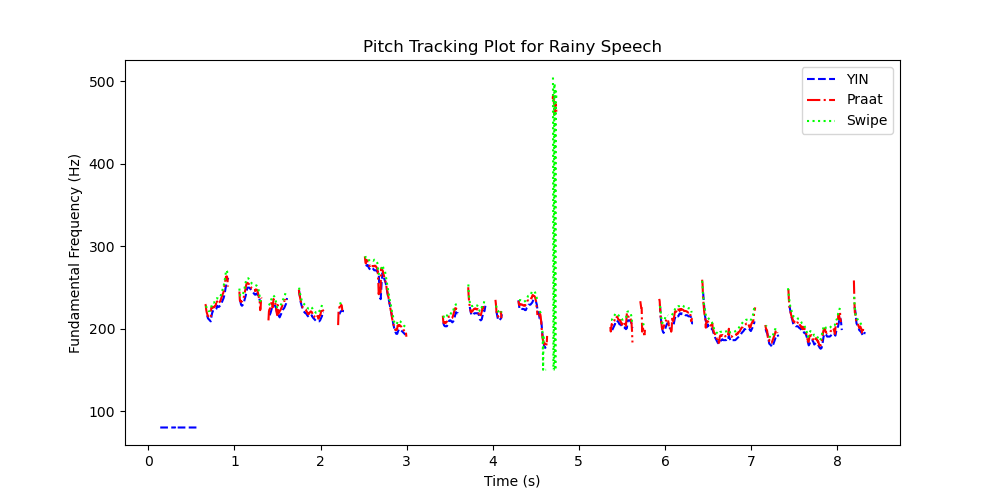
\includegraphics[width=0.8\linewidth]{recording4_rainy_fm_pitch_plot.png}
    \caption{Rainy Speech}
    \label{fig:enter-label}
\end{figure}

\textbf{Observations:}
\begin{itemize}
    \item \textbf{Praat's plot:} Praat shows a fair amount of consistency, with a contour that roughly follows a coherent pattern throughout the recording. Overall, Praat seems to be less robust against the type of noise that "rain" introduces, because among them, Praat has more out-of-range scatter points than the other two algorithms.Also, there are some intense deviations which are significantly out of range.



    \item \textbf{SWIPE's Plot:} SWIPE's performance is variable and shows some alignment with Praat's output, even the mistakes they made are the same in high frequency. But it also exhibits outliers and segments when the frequency is low, a couple of points just lower than trend.



    \item \textbf{YIN's Plot:} YIN's output here is quite consistent in most cases, except for the beginning, where it has detected an extremely low pitch that is likely not present in the actual speech. This could indicate that the algorithm is mistaking the low-frequency noise from the rain as speech.


\end{itemize}

\textbf{Summary:} In the presence of background noise like rain, Swipe appears to be the most reliable, as it maintains a stable pitch contour despite the noise. It may be filtering out the low-frequency noise more effectively. YIN is overly sensitive to the rain noise, which needs preprocessing to remove such consistent background noise. Swipe is the most stable and has the fewest deviation points and I suppose this algorithm is the most effective way to handle the "rainy" noise, while YIN and Praat may require additional strategies to mitigate the impact of background noise.\\

\textbf{Noisy speech:}
\begin{figure}[h]
    \centering
    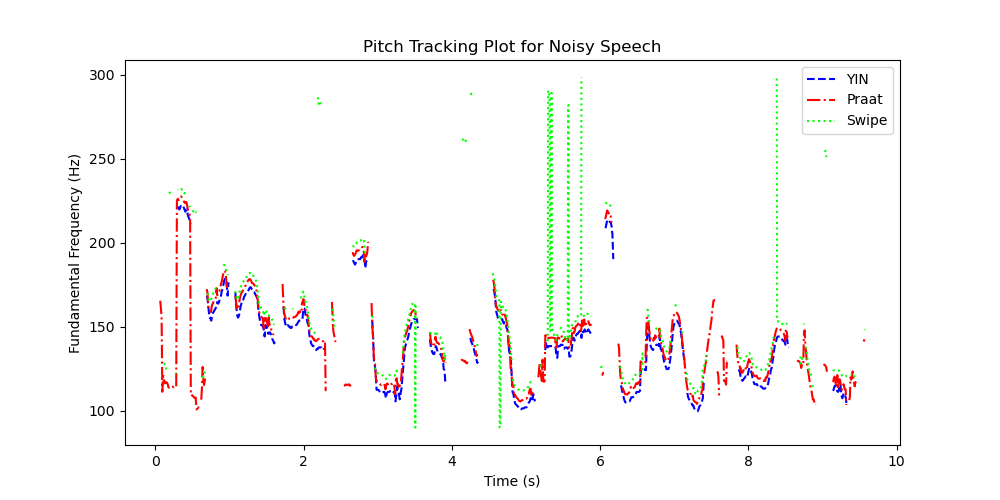
\includegraphics[width=0.8\linewidth]{recording5_noisy_m_pitch_plot.png}
    \caption{Noisy Speech}
    
\end{figure}

\textbf{Observations:}
\begin{itemize}
    \item \textbf{Praat's plot:} Praat captures the main underlying pattern of the targeted F0 as well as reserves the fine details where noise mixed up with speech. 




    \item \textbf{SWIPE's Plot:} SWIPE, as with the previous cases, displays a high degree of variation and some extreme outliers. In noisy conditions, this could indicate a high sensitivity to non-pitch elements of the sound, such as transient noise bursts or harmonic distortion. And some of these background elements are also perceived as speech. 



    \item \textbf{YIN's Plot:} YIN shows least dots in the graph as providing least data for  capturing F0. It suggests its conserveness in distinguishing sound in a noisy environment. Compared with the other two algorithms, it only depicts the main underlying pitch pattern while ignoring the uncertainties where noise mixed with speech. 



\end{itemize}

\textbf{Summary:} Praat seems to be more stable and consistent in noisy environments and is thus recommended. YIN and SWIPE react to the noise in 2 opposite directions, one is too conservative, leading to losing necessary information related to speech signal while the other one is too sensitive and reserves undesired f0 of noise, resulting in greater fluctuations.

\end{solution}

\bigskip
\textbf{References}:

\noindent De Cheveign\'e, A., \& Kawahara, H. (2002). YIN, a fundamental frequency estimator for speech and music. The Journal of the Acoustical Society of America, 111(4), 1917-1930

Talkin, D., \& Kleijn, W. B. (1995). A robust algorithm for pitch tracking (RAPT). Speech coding and synthesis, 495, 518.

Camacho, A., \& Harris, J. G. (2008). A sawtooth waveform inspired pitch estimator for speech and music. The Journal of the Acoustical Society of America, 124(3), 1638-1652.

Talkin, D. 2015. https://github.com/google/REAPER

Zahorian, S. A., \& Hu, H. (2008). A spectral/temporal method for robust fundamental frequency tracking. The Journal of the Acoustical Society of America, 123(6), 4559-4571.

\end{document}
